% !TEX encoding = UTF-8 Unicode
\documentclass[fleqn,twoside]{article}
\usepackage[ngerman]{babel}
\usepackage[utf8]{inputenc}
\usepackage[T1]{fontenc}
\usepackage{graphicx}
\usepackage{fancyhdr}
\usepackage{amssymb}
\usepackage{amsmath}
\usepackage{cite}
\usepackage{eurosym}
\usepackage{wrapfig}
\usepackage{tabularx}
\usepackage{pdfpages}
\usepackage{nicefrac}
\usepackage{wasysym}
\usepackage{multirow}
\usepackage{pifont}
\usepackage{textcomp}
\usepackage{comment}
\usepackage{units}
\usepackage{siunitx}
\usepackage{yfonts}
\usepackage{calligra}
\usepackage{csquotes}
%\usepackage{emerald}
\usepackage{titlesec}
\usepackage{tikz}
\usepackage{stanli}
\usepackage{romanbar}
\usepackage{graphicx}
\usepackage{tabto}
\usepackage{todonotes}
%\usepackage{3dstructuralanalysis}
%\usepackage{structuralanalysis}

%Betragsfunktion
\newcommand{\abs}[1]{\ensuremath{\left\vert#1\right\vert}}

\newcommand{\un}[2]{{\unit[#1]{\color{black!100}[#2]}}}

\usepackage[pdftex, colorlinks, linkcolor=black, frenchlinks]{hyperref}
\usepackage[a4paper , lmargin = {2.5cm} , rmargin = {2cm} , tmargin = {2.5cm} , bmargin = {2.5cm} ]{geometry}
\pagestyle{fancy}

\title{\Huge{\textfrak{Theoretische Bodenmechanik\\ mit} \textit{Mathematica}\textfrak{ \\Formelsammlung}}}
\author{\calligra{Jonathan C. Walter, Jonas H. Konrad}}
\date{\textfrak{\today}}

\begin{document}
\parindent 0pt
\fancyhead[L]{Jonathan C. Walter, Jonas H. Konrad}
\fancyfoot[L]{\frakfamily J. C. W.;J. H. K.}
\fancyfoot[R]{\frakfamily }
\fancyfoot[C]{\frakfamily Wir machen mit Mathematica \\Seite \thepage}
\maketitle \thispagestyle{empty}
%\initfamily %Für Initialien
\begin{center}
\textfrak{Diese Formelsammlung wurde im Sommersemester 2022 von Jonathan Walter und Jonas Konrad verfasst.\\Kein Anspruch auf Vollständigkeit oder Fehlerfreiheit.}
\end{center}
\tableofcontents
\listoftodos
\newpage

\section{Übersicht allgemeine Formeln/Umrechnungen}

%\subsection{Einheitenumrechnung}

%\begin{itemize}
%\item $Nm = \unit{\frac{kg \cdot m}{s^{2}}}$
%\end{itemize}

\subsection{Allgemeine Annahmen/Gesetzmäßigkeiten}

\begin{itemize}
\item Ablauf Spannungsverlauf:
	\begin{enumerate}
		\item Boden mit vorhandenen Spannungen
		\item Nach Probeentnahme: $\sigma^{ges}=u+\sigma = 0$ ; $\sigma$ unverändert
		\item Nach Einbau in Triax und schneller Belastung (undräniert): $\sigma$ unverändert ; $\sigma^{ges}$ = vorhandene Spannung + vorgegebener Wert ; $u=\sigma^{ges}-\sigma$
		\end{enumerate}
\item Bei langsamer Scherung im Wasserbad (dräniert) baut sich kein Porenwasserdruck auf: $u$ = 0
\item $K_0 = 1$ statt $K_0=1-\sin(\varphi)$ als legitime Annahme bei überkonsolidierten Boden 
\end{itemize}

\subsection{Allgemeine Formel für Klausuraufgaben}

\begin{enumerate}
\item Bodenparameter $\gamma$, $\gamma'$ und Kohäsion\\
		$e=\frac{w \gamma_s}{\gamma_w}$ ; w = Wassergehalt in \%\\
		$\gamma' = \frac{(\gamma_s-\gamma_w)}{(1+e)}$ oder $\gamma' = \gamma - u$\\
		$\gamma = \gamma'+\gamma_w$\\
		$C$ =  Fläche oder Länge (3D/2D) $\cdot$ $c_u$\\
		$OCR$ = $\frac{\sigma_V}{ \sigma}$ ; $\sigma_V$ = Vorbelastungsspannung ; $\sigma$ = effektive Spannung\\
		Bruchwinkel Abschätzung: $\vartheta = 45 - \frac{\varphi}{2}$
\item Bodenparameter mitteln\\
		Kohäsion: $\overline{c} = \frac{h_1 c_U + h_2 c_T}{\sum h_i}$\\
		Reibung: $\overline{\tan \varphi} = \frac{G_1 \tan(\varphi_U) + G_2 \tan(\varphi_T)}{G_1 + G_2}$\\
		Wichte: $\overline{\gamma} = \frac{G_1 + G_2}{\sum A_i}$
\item Effektive (Anfangs-)Vertikalspannung:\\
		$\sigma_{v0} = h_{\gamma} \cdot \gamma + (z-h_{\gamma})\gamma' + h_c \gamma_w $ ; $z$ = Tiefe der gesuchten Spannung\\
		Effektive (Anfangs-)Horizontalspannung:\\
		$\sigma_{h0} = K_0 \sigma_v$\\
		Anfangsporenwasserdruck:\\
		$u_0 = (z-z_{GWSp}) \cdot \gamma_w$\\
		Gesamtspannung:\\
		Vertikal und Horizontal zu Spannung aus Erddruck Porenwasserdruck addieren
\item Dissipationsenergie Verformung Boden\\
		$E=R\cdot s$ ; $s$=Deformationstiefe ; $R$=[S.78-Bodenmechanik]; $E = m\cdot g\cdot h$
\item Winkler-Setzung\\
		$k_s=\frac{\sigma_0}{s}$\\
		Dabei gespeicherte Energie: $E^{el}=\frac{1}{2}\cdot B\cdot L\cdot k_s\left[\frac{R}{B\cdot L\cdot k}\right]^2$ (Bsp. Rechteckfundament)
\item Prandtl-Lösung: Streifenfundament auf $c_u$-Boden:\\
		$P=(2+\pi)c_u B$ ; $P$=Auflast; $B$=Auflastbreite; Alternativ: $p=(2+\pi)c_u$\\
		Doppelamplitude: $q^{ampl}=2c^{ampl}_u$
\item 	Allgemeine Formel Triaxialversuch:\\
		Grundsätzlich gilt: triaxiale Kompression $\rightarrow$ $M_C$ ist maßgebend\\
		\phantom{Grundsätzlich gilt:} triaxiale Extension $\rightarrow$ $M_E$ ist maßgebend
		\begin{itemize}
		\item $\dot{p}^{ges}=\frac{1}{3}(\dot{\sigma}_1^{ges}+2\dot{\sigma}_3^{ges})$
		\item $\abs{\dot{q}}=\abs{\dot{\sigma}_1-\dot{\sigma}_3}$
		\item $\dot{u}\approx B\dot{p}^{ges}+A \abs{\dot{q}}$
		\item $\Delta p$ und $\Delta q$ berechnen: $A$ und $B$ bekannt, $p,q,u$ ebenso:\\
		$\Delta p = (1-B) \frac{1}{3} \Delta q-A\Delta q$\\
		$q+ \Delta q = M_c(p+\Delta p)$\\
		$\boxed{\Leftrightarrow \Delta q=\frac{q-M_cp}{M_c\left(\frac13(1-B)-1\right)-1}}$
		\item Kohäsion aus A und B berechnen\\ 
		\begin{minipage}{0.5\textwidth}
		Berechnung:\\
		Bekannte Steigung aus $\varphi_s \rightarrow M_c=(6s)/(3-s)$\\
		$M_{c,neu}$ vorgehen:\\ 
		1. $M_{c,\text{vorläufig}} = \Delta_{s}(aus \varphi_s) \cdot A$\\ 
		2. $M_{c,neu} = \dfrac{\Delta_{s,\text{Zähler} \overset{!}{=} 1} - \Delta_{s,\text{Nenner}} \cdot B}{\Delta_{s,\text{Nenner}}}$\\
		3. Ab $p = \sigma_{a0}$ auftragen\\
		4. Schnittpunkt aus $M_c = M_{c,neu}$ berechnen.\\
		5. $c_u = \frac{q}{2}$ 
		\end{minipage}		
		\begin{minipage}{0.5\textwidth}
		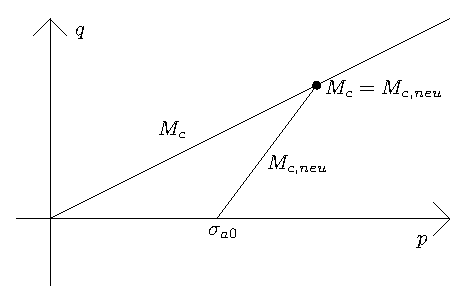
\includegraphics[width=0.7\textwidth]{IPE/Konstruktion_c_u_aus_A&B/Graphische_Version.eps}
		\end{minipage}
		\item Abschätzung maximale Schubspannung: $c_u = \tau_{\max} = \sigma_V \tan(\varphi)$\\
		$\sigma_V$ aus Angabe Belastung Knick nehmen.
		\item Restscherfestigkeit: $\tau = \sigma \tan(\varphi_s)$ ; $\sigma$ aus in-situ
		\item Winkel Gesamtscherfestigkeit: $\sin(\varphi_s)=\frac{\sigma_1-\sigma_3}{\sigma_1+\sigma_3}$ ; mit effektiver Spannung berechnen!
		\item Undrainierte Schubsteifigkeit: $G= \frac{\Delta q}{3 \Delta \epsilon_q}$
		\item Volumendehnung: $\epsilon_{vol}=\epsilon_1 + 2\epsilon_3$
		\item Deviatorische Dehnung: $\epsilon_q = \frac{2}{3}(\epsilon_1 - \epsilon_3)$\\
		$\rightarrow$ Bei undränierten Versuchen gilt: $\epsilon_{2(3)}=-\frac{\epsilon_1}{2}$
		\end{itemize}
\item Anstieg Porenwasserdruck aus zyklischer Belastung: (nach Skempton)\\
		Ermittlung Parameter:\\
		$B = \frac{\Delta u}{\Delta p^{ges}}$ ; aus B-Test\\
		$\rightarrow$ B beschreibt Qualität der Sättigung. Perfekt gesättigte Triaxialproben: $B = 1$\\
		$A  = \frac{\Delta u - B \Delta tr\sigma^{ges}}{\Delta q}$ ; $\sigma_1$ oder $\sigma_3$ steigen an\\
		$\tab$ $\Delta q = \Delta q_{1,2 Ende}-\Delta q_{1,2 Anfang}$ \\
		$\tab$ $\Delta tr\sigma^{ges} =\Delta p= \frac{\sigma_1 +2\cdot \sigma_3}{3}_{(Zustand 1)} - \frac{\sigma_1 +2\cdot \sigma_3}{3}_{(Zustand 2)} $\\
		Für $p^{ges}$ = const. $\rightarrow$ pro Zyklus $\Delta u=2Aq^{ampl} = 2A(\Delta \sigma^{ges}_v - \Delta \sigma^{ges}_h)$ \\
		Für $q$ = const. $\rightarrow$ pro Zyklus $\Delta u=B\Delta p^{ges}$
\item Konsolidierung - Dissipationszeit Porenwasserüberdruck\\
		Barotrope Steifigkeit: $E_s=\frac{\sigma_{v0}}{\kappa}$\\
		Konsolidierungsbeiwert: $c_v=\frac{kE_s}{\gamma_w}$\\
		Dimensionsloser Zeitfaktor: $T_v=\frac{c_vt}{H^2}$ ; $\un{t}{s}$; $\un{h}{m}$; $H$ = Drainageweg Wasser ; \\
		Verfestigungsgrad: $\bar{\mu}\approx 2 \cdot \sqrt{T_v/\pi}$\\
		Konsolidierungsgrad: $\mu=\frac{1}{2}(3\bar{\mu}-1)$ ; Faktor Verfestigung Boden nach t Sekunden aus $T_v$\\
		Aufgebauter Porenwasserdruck nach $n$ Zyklen$\cdot$Konsolidierungsgrad \\= Porenwasserdruck nach t$\cdot$n Wartezeit; 
		$(\Delta u \cdot n) \cdot \mu = \Delta u_{konsolidiert}$
\item Tresca Kiriterium\\
		$2c_u = (\sigma_{\max}-\sigma_{\min})=(\sigma_{\max}^{ges}-\sigma_{\min}^{ges})$
\item Coulomb-Kriterium\\
		$(\sigma_{\max}-\sigma_{\min})=(\sigma_{\max}+\sigma_{\min})\sin(\varphi)+2c\cos(\varphi)$\\
		oder\\
		$\sqrt{(\sigma_{11}-\sigma_{22})^2+4\sigma^{2}_{12}}=(\sigma_{11}+\sigma_{22})\sin(\varphi)+2c\cos(\varphi)$
\item Roscoe Invarianten (Druck $p$ und Deviatorspannung $q$) ; ohne Wasserdruck!\\
		$p=\frac{\sigma_1+2\cdot\sigma_3}{3}$ , Auch für $\Delta p^{ges}$ verwenden.\\
		$q=\sigma_1-\sigma_3 \widehat{=} 2 \cdot c_u$\\
		$M_C=\frac{q}{p} = \frac{6s}{3-s}$ ; $s=\sin(\varphi_s)$ ; $\eta$ beschreibt Steigung Schergerade in $p$ - $q$ Diagramm \\
		$\rightarrow$ (dafür die gesamten Spannungen mit abgezogenen $u_0$ verwenden)\\
		Daraus ergibt sich: $2c_u=\frac{6 \cdot \sin(\varphi)}{3-\sin(\varphi)} \cdot p$\\
		Spannungspfad startet bei: $p_0 = \frac{1}{3} (1+2K_0)\sigma_0$ ; für $\sigma_v^{ges},\sigma_h^{ges}$ durchführen.\\
		Für Startpunkt der zyklischen Belastungen die effektive Spannung ($\sigma_v^{ges},\sigma_h^{ges}$) im Boden benutzen)\\
		$A$ gibt Steigung von -$p$ Sprung an, $q^{ampl}$ die Höhe.
\item Krey-Tiedemann Modell:\\
		$c_u \approx \sigma'_{VB} \tan(\varphi_s)$\\
		$w(z)= \frac{\rho_w V_p}{\rho_s V_s}=e \frac{\rho_w}{\rho_s}$
\item Strömungskraftdichte und Porenwasserüberdruck\\
		Hydraulischer Gradient: $i=\frac{w}{k}$\\
		\hspace*{1cm} Gradient bei $\Delta h$ des GWSp mit zwei versch. Schichten.\\
		\hspace*{1cm} $w=k_U i_U = k_T i_T$ ; $i_T = \frac{k_U}{k_T} L_T$ ; $i_U = \frac{\Delta h}{L_U + \frac{k_U}{k_T}L_T}$\\
		Strömungskraftdichte: $j= \gamma_w \cdot i$\\
		Gewicht mit Strömungskräfte (Auftrieb):$G = A_1 \cdot (\gamma' - j_1) + A_2 \cdot (\gamma' - j_2)$\\
		Porenwasserüberdruck auf Körper (in Mittelpunkt der Gleitfläche): $u^+=i\gamma_wx_1$
\item Kompressionsdiagramm auswerten (Abszisse: $\sigma$ ; Ordinate: 1+$e$ \autoref{Scherversuch} [siehe 1.]) \\
		$\kappa_B = \log(\frac{(1+e)_1}{(1+e)_2}) = -\kappa \log(\frac{\sigma_1}{\sigma_2})$ $\rightarrow$ Auf oberen flachen Teil durchführen\\
		$\lambda_B = \log(\frac{(1+e)_1}{(1+e)_2}) = -\lambda \log(\frac{\sigma_1}{\sigma_2})$ $\rightarrow$ Auf steilen Teil durchführen\\
		Für Punkt z den Wert $e$ berechnen; $\sigma$ aus Diagramm ablesen; $c_u = \sigma_{VB} \tan(\varphi_s)$\\
		Analytische Lösung: $ln[e/e_{e0}]$ = $\lambda_B \text{ln}[\sigma_{VB} / \sigma_{e0}]$ ; 
							$ln[e/e(z)]$ = $\kappa_B \text{ln}[\sigma_{VB} / \sigma(z)]$ 
\item Kräftegleichgewicht
		\begin{enumerate}
		\item Mit Strömungskraft\\
				Eigengewicht: $G=\gamma' \cdot V$\\
				Strömungskraft: $F_s=j \cdot V$
		\item Mit Porenwasserdrücken\\
				Eigengewicht: $G=\gamma \cdot V$\\
				Hydrostatischer Anteil der Porenwasserdrücke: $U=\gamma_w \cdot V$\\
				Porenwasserüberdrücke: (Summe über Ränder) $U^+=j \cdot V$
		\item Für beide Fälle zu verwenden:\\
				Reaktionskräfte: Q\\
				Zwischenkräfte: $E_{12}$\\
				Äußere Belastungen\\
		\end{enumerate}
\item Mohr'scher Spannungskreis\label{Scherversuch}\\
		
		\begin{minipage}{0.3\textwidth}
		Allgemeine Formeln:\\
		$\sigma_{11}=x \cdot \gamma' \cdot \beta$\\
		$\tau = \sigma_{11}  \cdot \frac{\sigma}{\sigma'} \cdot \tan(\beta)$\\\\
		Ablauf Krey-Tiedemann:
		\begin{enumerate}
		\item $\varphi_s$ auftragen
		\item $\sigma_{VB}$ auftragen und bis $\varphi_s$ verlängern
		\item An Schnittpunkt $\varphi '$ ansetzen und nach links einzeichnen
		\item mit $\varphi$ und $\alpha$ den Schnittpunkt mit $\varphi_s$ bestimmen.
		\item Dieser Punkt ist $\tau_{\max}$ und mit dem gegebenen $\sigma$ wird ein Kreis innerhalb der $\varphi '$ konstruiert.
		\item Schnittpunkt rechte Seite Kreis mit Abszisse ist $\sigma_1$
		\end{enumerate}
		\end{minipage}		
		\begin{minipage}{0.6\textwidth}
		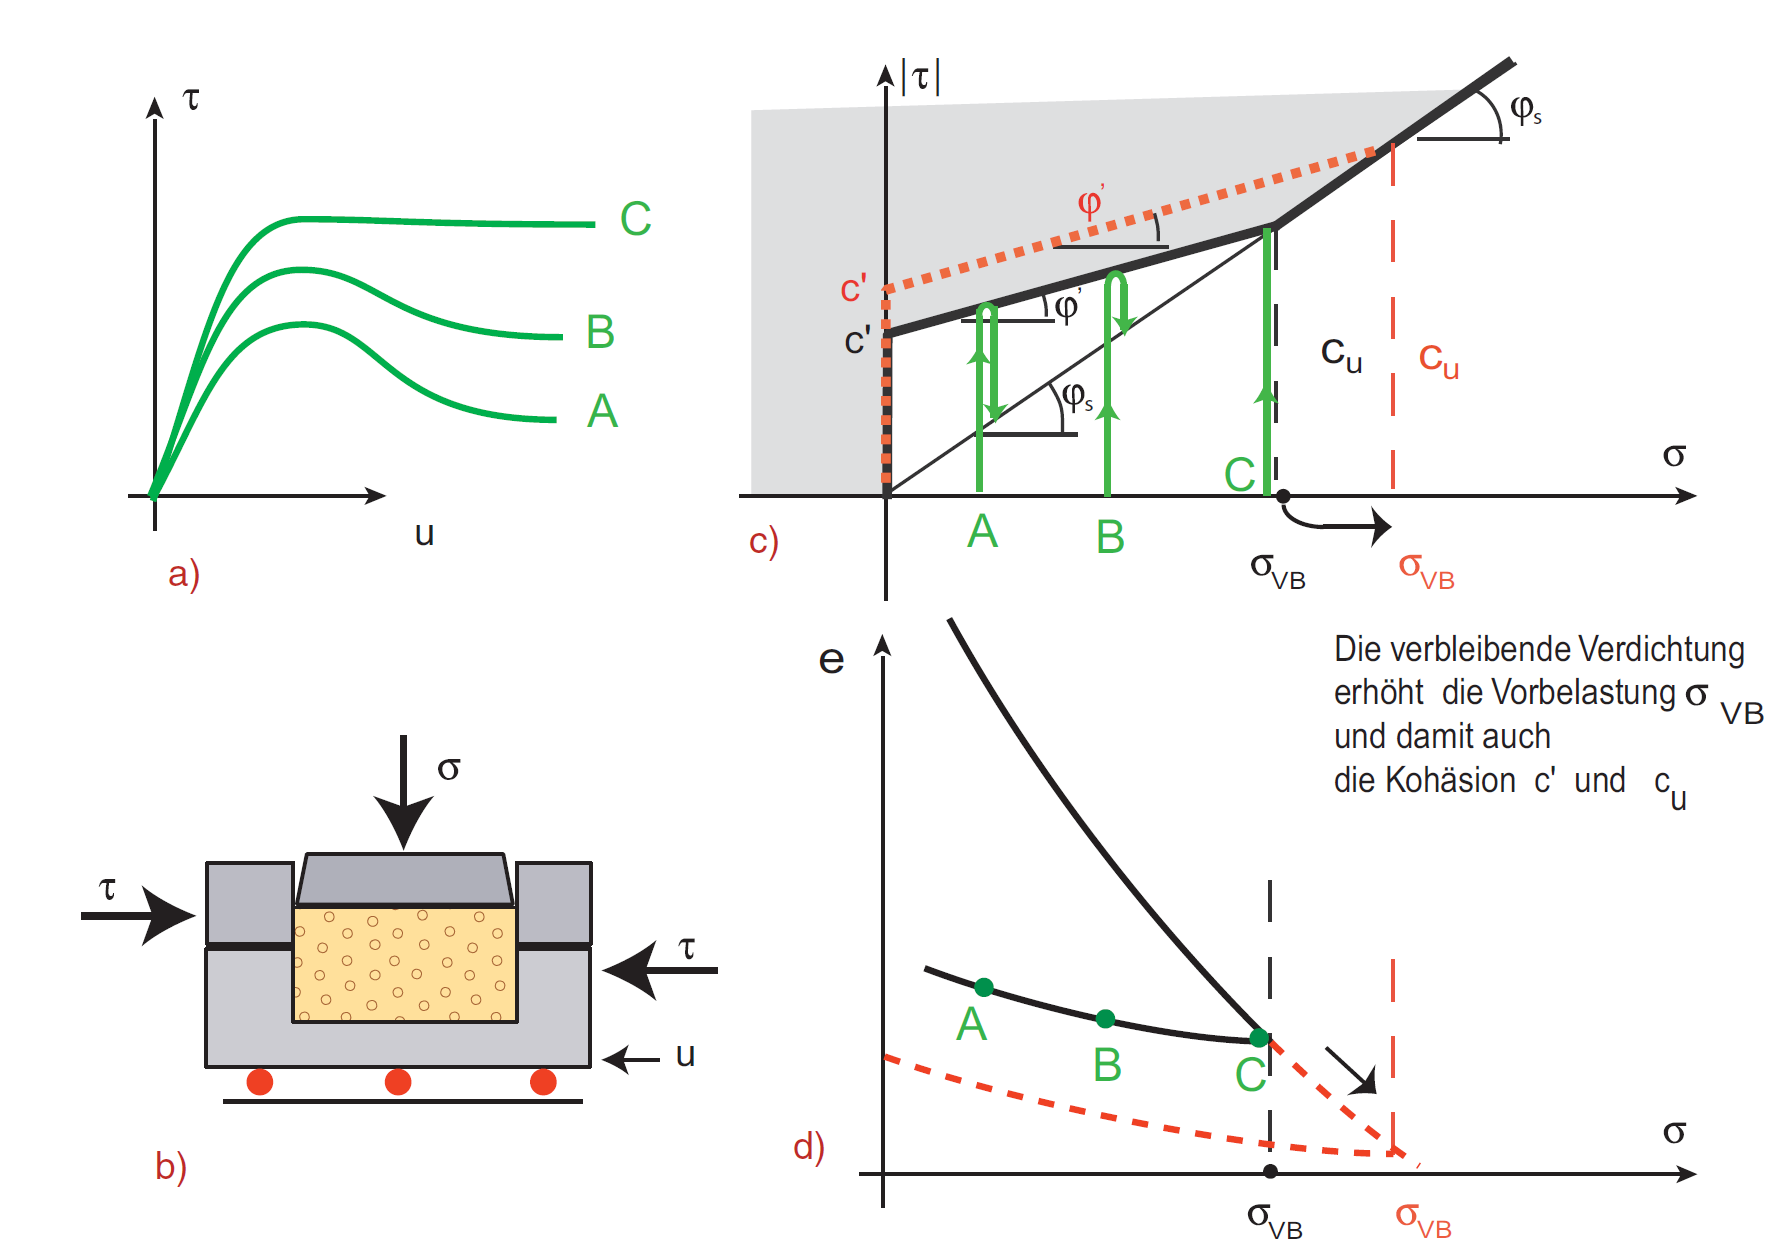
\includegraphics[width=1.1\textwidth]{Grafiken/Krey-Tidemann-Kriterium.png}
		\end{minipage}
\item Dissipationsenergie D\\
		$D= \abs{ [[ v_t^k ]] } \cdot (c + \sigma_{nn} \tan(\varphi) - \sigma_{nn} \tan(\psi)>0$ , wobei gilt: $[[ v_t ]] = \cos(\alpha)$\\
\item Schräghangaufgabe:\\
		Spannungsberechnung: ($x_1$ = senkrecht zu Hang gemessen)\\
		$\sigma_{11} = x_1 \gamma' \cos(\beta) + \gamma_w \cdot h_c$\\
		\hspace*{1cm} $h_c = z \cdot \cos(\beta)^2$\\
		$\sigma_{21} = x_1 \cdot \gamma \cdot \sin(\beta)$\\
		Erforderlicher Reibungswinkel: $\varphi_{erf} = \arctan(\frac{\sigma_{21}}{\sigma_{11}})$	
		
\item Kriechhang, Verdübelung, Verankerung:\\
		\begin{itemize}
		
		\item Grundlegende Formeln:\\
		Schubfestigkeit oberhalb Kontaktfläche (ohne Verdübelung):\\
		\hspace*{1cm} $\tau_\alpha = F_1 + G_1 \sin(\beta)$\\
		\hspace*{1cm} G = Gewicht einer vertikalen Bodensäule mit Einheitsfläche 1 m$^2$ gemessen entlang der\\ 
		\hspace*{1cm} Böschung (und nicht horizontal); F = Sickerkraft in dieser Bodensäule.\\
		\hspace*{1.5cm} z.B.: $\tau_\alpha = \gamma_w h \cos(\beta) \sin(\beta) + h \gamma' \cos(\beta) \sin(\beta)$\\
		\hspace*{1cm} Diese Festigkeit gilt als Referenz über die gesamte Höhe.\\
		\hspace*{1cm} Rest müssen über Dübel (Höhe h und Druchmesser D)abgetragen werden.\\
		Nach Leinenkugel (an Sohle): $\tau = \tau_\alpha (1+ I_v \ln(\frac{1}{\text{n-fach langsamer}})$\\
		Restliche Schubkraft pro 1m$^2$ der Oberfläche übernehmen die Dübel:\\ 
		\hspace*{1cm}$\tau_D = \tau_\alpha - \tau = \tau_\alpha I_v \ln (\text{n-fach langsamer})$\\
		Kraft pro Dübel: $p_f \cdot h$\\
		\hspace*{1cm} $p_f = \left[1+I_v \ln \frac{v_{red} / (a-D)}{\dot{\gamma_a}}\right] k_0 c_{u\alpha} D$ ; $k_0 = 4,83 \cdot \left[ 2,76 \frac{D}{a}+1 \right]$\\ 
		\hspace*{1cm} a = axialer Abstand quer zur Hanglinie\\
		Verformungsrate: $\dot{\gamma}_\alpha = \frac{v}{h_\gamma \cos(\beta)}$ ; $h_\gamma$ = h über Kontaktfläche in der kriechenden Schicht.\\
		Schlussendlich: $p_f \cdot h = h \left[1+I_v \ln \frac{v_{red} / (a-D)}{\dot{\gamma_a}}\right] k_0 c_{u\alpha} D = \tau_D a L$ ; $c_{u\alpha}=\tau_\alpha$
		
		\item Verdübelung eines Hangs:\\
		(h=Höhe Gleitscholle, B=Breite der Zone, D=Durchmesser eines Dübels)\\
		Referenzkohäsion: $c_{u\alpha}=W\sin(\beta)$ ; $W=\gamma h \cos(\beta)$\\
		Wirkung der Verdübelung pro lfm der Böschungslinie (ohne Seitenkräfte): \\ 
			\hspace*{1cm} $P_f=B(c_{u\alpha}-c_u)=B(I_V \cdot c_{u\alpha} \cdot \ln(0,1))$\\
		Schubkräfte auf den Seiten: $H=2 \cdot 0,1 \cdot c_{u\alpha} h \cos(\beta)$\\
		Notwendige Kohäsion: $c_{u,\text{erf}}=\frac{WB\sin(\beta)-P_f+H}{B}$\\
		Kriechrate des Hangs in der verdübelten Zone:\\ \hspace*{1cm} $c_{u,\text{erf}} - c_{u\alpha} = I_V c_{u\alpha} \ln(v/v_\alpha)$ ; 
			 $v=v_\alpha \exp\left[\frac{c_{u,\text{erf}}-c_{u\alpha}}{I_Vc_{u\alpha}}\right]$\\
		Sicherheitsabstand für Knopflochlösung: $x=v\cdot t$\\
		
		\item Ausführung mit Vakuum-Vorbelastung:\\
		$I_V$ berechnen: $\frac{\dot{\gamma}_a}{\dot{\gamma}_b} = (\frac{c_{ua}}{c_{ub}})^{1/I_V}=(\frac{\tau_{ua}}{\tau_{ub}})^{1/I_V}$ ; $\dot{\gamma}_{a,b}$ = Verformungsraten Boden vorher/nachher\\
		OCR berechnen: OCR = $\frac{\sigma_{11}+\Delta \sigma_{11}}{\sigma_{11}}$\\
		n-fache Bremsung der Kriechrate: $n = (\frac{OCR_a}{OCR_b})^{-1/I_V}= (\frac{1}{OCR})^{-1/I_V}$\\
		Normale Komponente nach der Belastung: $\sigma_{11,nachher}=\sigma_{11} \cdot OCR$\\
		Schubkomponente: $\sigma_{21} = \sigma_{11} \cdot \sin(\beta)$\\
		$\sigma_n = \sqrt{\sigma_{11}^2 + \sigma_{21}^2}$\\
		$m=\frac{\sigma_n}{\cos(\beta)}$ ; $r=\sigma_n \cdot \tan(\beta)$ ; $\sigma_1=m+r$ ; $\sigma_2=m-r$ ; $\sigma_3 = \sigma_2$\\
		$p=\frac{(\sigma_1+\sigma_2+\sigma_3)}{3}$ ; $q=\sigma_1-\sigma_2$\\
\begin{figure}[ht]		
		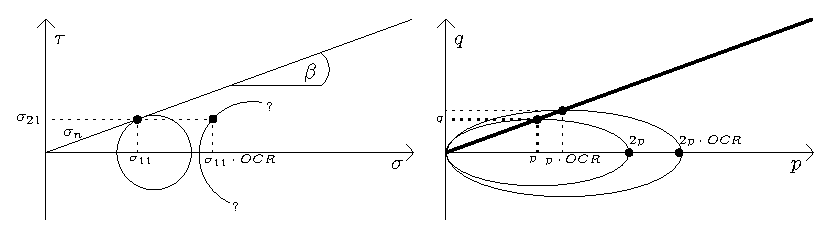
\includegraphics[width=0.8\textwidth]{IPE/Konsolidierung_Kriechhang/Konsolidierung_Kriechhang.eps}
		\caption{Links: Mohr'scher Kreis vor und während der Vorbelastung.\\ 
		Rechts: Spannungszustand und Vorbelastungsflächen vor und nach der Vorbelastung}
\end{figure}

		\end{itemize}
	


\end{enumerate}

\end{document}
